\documentclass[14pt]{extbook}
\usepackage{multicol, enumerate, enumitem, hyperref, color, soul, setspace, parskip, fancyhdr} %General Packages
\usepackage{amssymb, amsthm, amsmath, bbm, latexsym, units, mathtools} %Math Packages
\everymath{\displaystyle} %All math in Display Style
% Packages with additional options
\usepackage[headsep=0.5cm,headheight=12pt, left=1 in,right= 1 in,top= 1 in,bottom= 1 in]{geometry}
\usepackage[usenames,dvipsnames]{xcolor}
\usepackage{dashrule}  % Package to use the command below to create lines between items
\newcommand{\litem}[1]{\item#1\hspace*{-1cm}\rule{\textwidth}{0.4pt}}
\pagestyle{fancy}
\lhead{Makeup Progress Quiz 3}
\chead{}
\rhead{Version A}
\lfoot{4315-3397}
\cfoot{}
\rfoot{Fall 2020}
\begin{document}

\begin{enumerate}
\litem{
Write the equation of the graph presented below in the form $f(x)=ax^2+bx+c$, assuming  $a=1$ or $a=-1$. Then, choose the intervals that $a, b,$ and $c$ belong to.
\begin{center}
    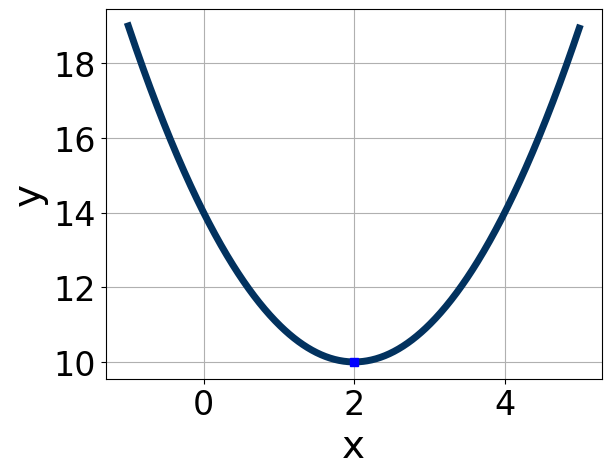
\includegraphics[width=0.5\textwidth]{../Figures/quadraticGraphToEquationA.png}
\end{center}
\begin{enumerate}[label=\Alph*.]
\item \( a \in [0, 2], \hspace*{5mm} b \in [-4, 3], \text{ and } \hspace*{5mm} c \in [12, 17] \)
\item \( a \in [-3, 0], \hspace*{5mm} b \in [2, 8], \text{ and } \hspace*{5mm} c \in [2, 10] \)
\item \( a \in [0, 2], \hspace*{5mm} b \in [2, 8], \text{ and } \hspace*{5mm} c \in [12, 17] \)
\item \( a \in [0, 2], \hspace*{5mm} b \in [2, 8], \text{ and } \hspace*{5mm} c \in [-7, -4] \)
\item \( a \in [-3, 0], \hspace*{5mm} b \in [-4, 3], \text{ and } \hspace*{5mm} c \in [2, 10] \)

\end{enumerate} }
\litem{
Solve the quadratic equation below. Then, choose the intervals that the solutions belong to, with $x_1 \leq x_2$ (if they exist).\[ -12x^{2} +13 x -2 = 0 \]\begin{enumerate}[label=\Alph*.]
\item \( x_1 \in [-0.17, 0.91] \text{ and } x_2 \in [0.5, 1.6] \)
\item \( x_1 \in [-11.47, -10.3] \text{ and } x_2 \in [-3.7, -1.4] \)
\item \( x_1 \in [-1.25, -0.73] \text{ and } x_2 \in [-0.6, 0.6] \)
\item \( x_1 \in [-8.58, -7.41] \text{ and } x_2 \in [8.7, 9.5] \)
\item \( \text{There are no Real solutions.} \)

\end{enumerate} }
\litem{
Factor the quadratic below. Then, choose the intervals that contain the constants in the form $(ax+b)(cx+d); b \leq d.$\[ 81x^{2} -9 x -20 \]\begin{enumerate}[label=\Alph*.]
\item \( a \in [7.3, 9.5], \hspace*{5mm} b \in [-8, -2], \hspace*{5mm} c \in [8.2, 9.3], \text{ and } \hspace*{5mm} d \in [-1, 5] \)
\item \( a \in [0.4, 1.5], \hspace*{5mm} b \in [-47, -38], \hspace*{5mm} c \in [0.9, 2.6], \text{ and } \hspace*{5mm} d \in [35, 39] \)
\item \( a \in [1.8, 3.8], \hspace*{5mm} b \in [-8, -2], \hspace*{5mm} c \in [26.4, 31.5], \text{ and } \hspace*{5mm} d \in [-1, 5] \)
\item \( a \in [24.8, 29.1], \hspace*{5mm} b \in [-8, -2], \hspace*{5mm} c \in [1.2, 3.3], \text{ and } \hspace*{5mm} d \in [-1, 5] \)
\item \( \text{None of the above.} \)

\end{enumerate} }
\litem{
Solve the quadratic equation below. Then, choose the intervals that the solutions belong to, with $x_1 \leq x_2$ (if they exist).\[ -10x^{2} -8 x + 5 = 0 \]\begin{enumerate}[label=\Alph*.]
\item \( x_1 \in [-1.4, -0.5] \text{ and } x_2 \in [0.35, 0.42] \)
\item \( x_1 \in [-17.9, -15.9] \text{ and } x_2 \in [15.7, 15.88] \)
\item \( x_1 \in [-5.3, -3.4] \text{ and } x_2 \in [11.91, 12.38] \)
\item \( x_1 \in [-0.9, -0.3] \text{ and } x_2 \in [1.03, 1.39] \)
\item \( \text{There are no Real solutions.} \)

\end{enumerate} }
\litem{
Solve the quadratic equation below. Then, choose the intervals that the solutions $x_1$ and $x_2$ belong to, with $x_1 \leq x_2$.\[ 8x^{2} -18 x -81 = 0 \]\begin{enumerate}[label=\Alph*.]
\item \( x_1 \in [-7.9, -3.5] \text{ and } x_2 \in [1.47, 1.59] \)
\item \( x_1 \in [-2.9, -0.9] \text{ and } x_2 \in [4.17, 4.68] \)
\item \( x_1 \in [-20.8, -17.6] \text{ and } x_2 \in [35.67, 36.03] \)
\item \( x_1 \in [-10.8, -8.1] \text{ and } x_2 \in [1.09, 1.28] \)
\item \( x_1 \in [-0.9, 1.8] \text{ and } x_2 \in [13.48, 13.85] \)

\end{enumerate} }
\litem{
Solve the quadratic equation below. Then, choose the intervals that the solutions $x_1$ and $x_2$ belong to, with $x_1 \leq x_2$.\[ 15x^{2} +2 x -24 = 0 \]\begin{enumerate}[label=\Alph*.]
\item \( x_1 \in [-2.02, -1.01] \text{ and } x_2 \in [0.82, 1.52] \)
\item \( x_1 \in [-0.8, -0.38] \text{ and } x_2 \in [3.47, 3.7] \)
\item \( x_1 \in [-2.71, -2.34] \text{ and } x_2 \in [0.41, 0.62] \)
\item \( x_1 \in [-4.21, -3.84] \text{ and } x_2 \in [0.14, 0.57] \)
\item \( x_1 \in [-20.22, -19.73] \text{ and } x_2 \in [17.84, 18.35] \)

\end{enumerate} }
\litem{
Graph the equation below.\[ f(x) = (x-4)^2 - 14 \]\begin{enumerate}[label=\Alph*.]
\begin{multicols}{2}\item 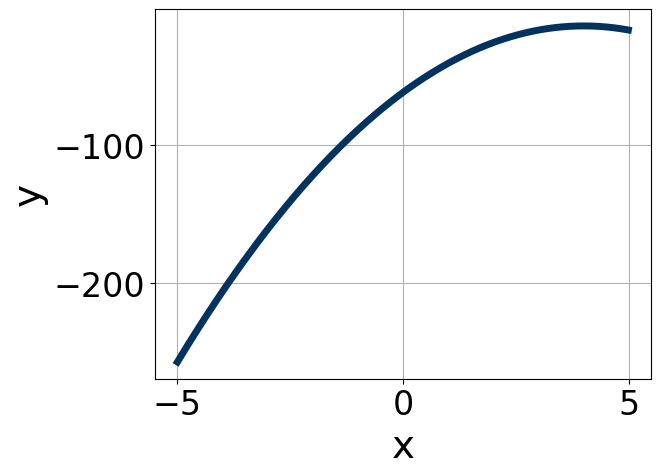
\includegraphics[width = 0.3\textwidth]{../Figures/quadraticEquationToGraphCopyAA.png}\item 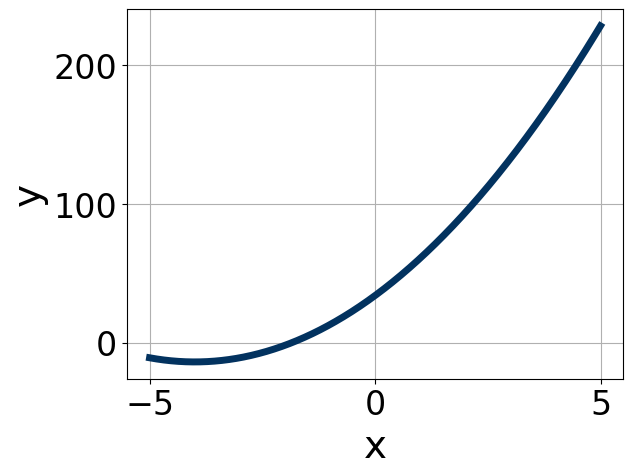
\includegraphics[width = 0.3\textwidth]{../Figures/quadraticEquationToGraphCopyBA.png}\item 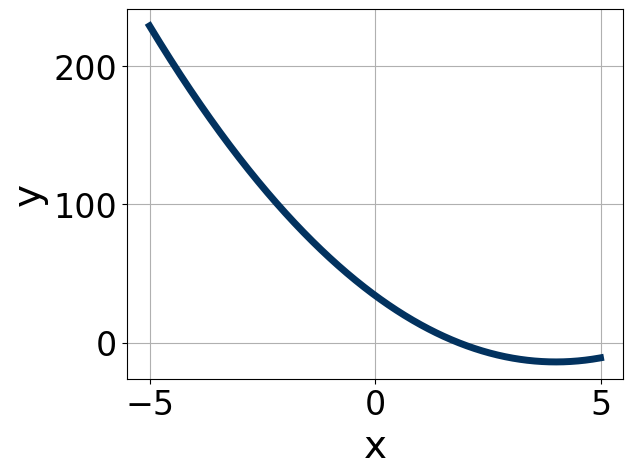
\includegraphics[width = 0.3\textwidth]{../Figures/quadraticEquationToGraphCopyCA.png}\item 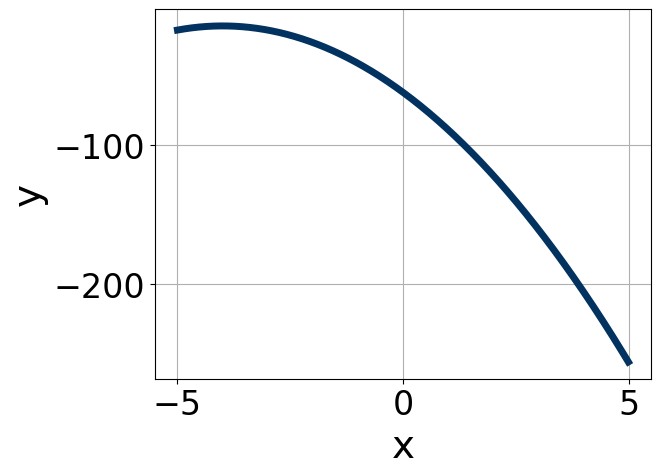
\includegraphics[width = 0.3\textwidth]{../Figures/quadraticEquationToGraphCopyDA.png}\end{multicols}\item None of the above.
\end{enumerate} }
\litem{
Factor the quadratic below. Then, choose the intervals that contain the constants in the form $(ax+b)(cx+d); b \leq d.$\[ 54x^{2} +57 x + 10 \]\begin{enumerate}[label=\Alph*.]
\item \( a \in [2.4, 3.5], \hspace*{5mm} b \in [-6, 5], \hspace*{5mm} c \in [17, 18.2], \text{ and } \hspace*{5mm} d \in [5, 9] \)
\item \( a \in [8.9, 9.8], \hspace*{5mm} b \in [-6, 5], \hspace*{5mm} c \in [5.8, 7.6], \text{ and } \hspace*{5mm} d \in [5, 9] \)
\item \( a \in [15.6, 20.4], \hspace*{5mm} b \in [-6, 5], \hspace*{5mm} c \in [1.4, 3.1], \text{ and } \hspace*{5mm} d \in [5, 9] \)
\item \( a \in [0.7, 2.7], \hspace*{5mm} b \in [12, 14], \hspace*{5mm} c \in [-1.4, 2.5], \text{ and } \hspace*{5mm} d \in [44, 49] \)
\item \( \text{None of the above.} \)

\end{enumerate} }
\litem{
Write the equation of the graph presented below in the form $f(x)=ax^2+bx+c$, assuming  $a=1$ or $a=-1$. Then, choose the intervals that $a, b,$ and $c$ belong to.
\begin{center}
    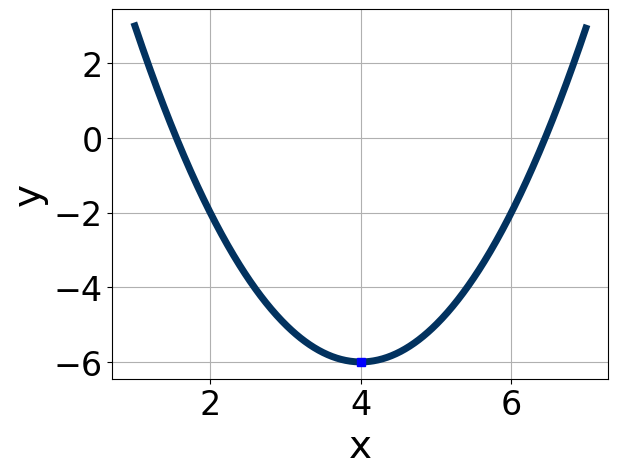
\includegraphics[width=0.5\textwidth]{../Figures/quadraticGraphToEquationCopyA.png}
\end{center}
\begin{enumerate}[label=\Alph*.]
\item \( a \in [-5, 0], \hspace*{5mm} b \in [-11, -6], \text{ and } \hspace*{5mm} c \in [-22, -20] \)
\item \( a \in [1, 4], \hspace*{5mm} b \in [5, 13], \text{ and } \hspace*{5mm} c \in [20, 25] \)
\item \( a \in [-5, 0], \hspace*{5mm} b \in [5, 13], \text{ and } \hspace*{5mm} c \in [-22, -20] \)
\item \( a \in [1, 4], \hspace*{5mm} b \in [5, 13], \text{ and } \hspace*{5mm} c \in [7, 11] \)
\item \( a \in [1, 4], \hspace*{5mm} b \in [-11, -6], \text{ and } \hspace*{5mm} c \in [7, 11] \)

\end{enumerate} }
\litem{
Graph the equation below.\[ f(x) = -(x+2)^2 + 13 \]\begin{enumerate}[label=\Alph*.]
\begin{multicols}{2}\item 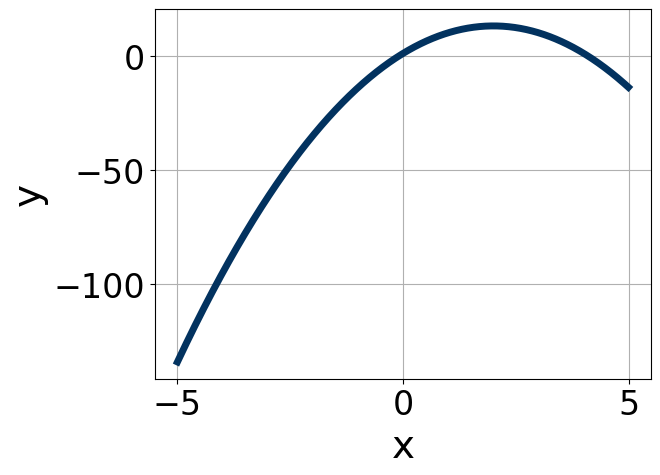
\includegraphics[width = 0.3\textwidth]{../Figures/quadraticEquationToGraphAA.png}\item 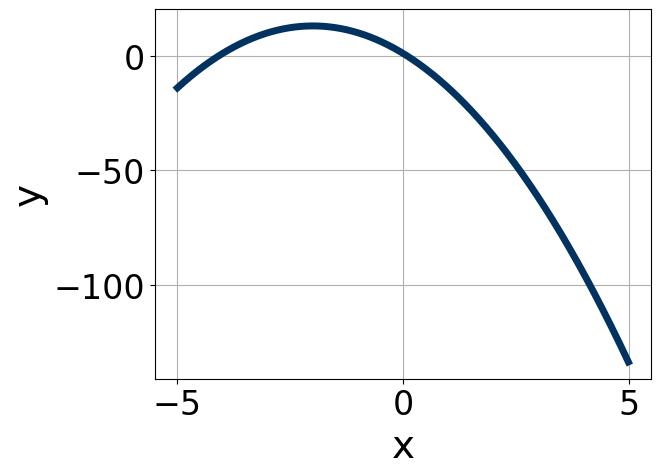
\includegraphics[width = 0.3\textwidth]{../Figures/quadraticEquationToGraphBA.png}\item 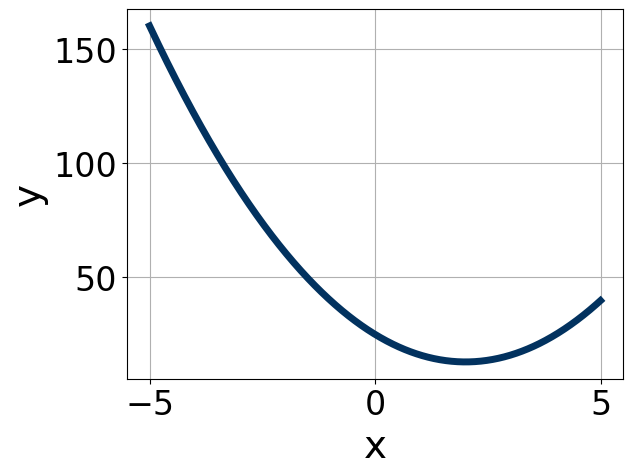
\includegraphics[width = 0.3\textwidth]{../Figures/quadraticEquationToGraphCA.png}\item 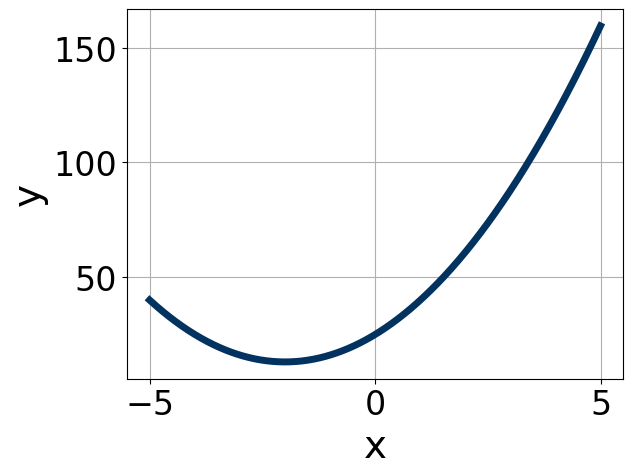
\includegraphics[width = 0.3\textwidth]{../Figures/quadraticEquationToGraphDA.png}\end{multicols}\item None of the above.
\end{enumerate} }
\end{enumerate}

\end{document}